\section{Image resolution}

Image resolution refers to the pixel density within a given physical unit, typically measured in DPI (Dots Per Inch). 
In the context of raster graphic devices, resolution is relative to the size of the monitor rather than being an absolute metric as in printed images. 
Consequently, the resolution of a screen specifies the number of pixels displayed horizontally ($s_w$) and vertically ($s_h$). 
It's important to note that pixels may not have a square shape, and as a result, the horizontal resolution often differs from the vertical resolution.

\subsection{Coordinates}
The coordinate system utilized is Cartesian, with the origin situated in the top-left corner. The $x$-axis progresses horizontally from left to right, while the $y$-axis ascends vertically from top to bottom.
\begin{figure}[H]
    \centering
    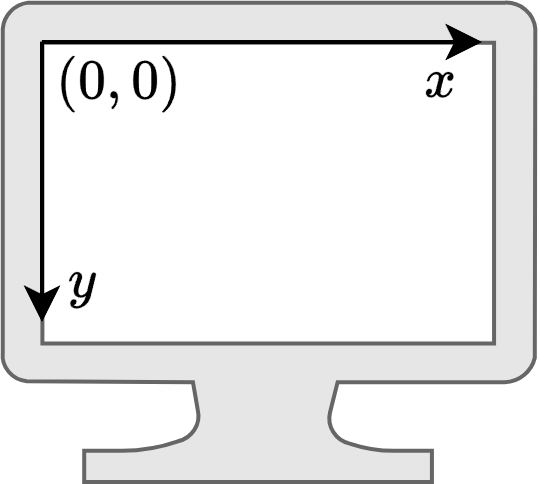
\includegraphics[width=0.25\linewidth]{images/coordinates.png}
    \caption{Pixel coordinates}
\end{figure}
The coordinate system adheres to a left-handed convention, signifying that the $y$-axis extends in the opposite direction compared to the conventional Cartesian system.
As a consequence, the integer values of $x$ and $y$ coordinates fall within the range:
\[0 \leq x \leq s_w-1\]
\[0 \leq y \leq s_h-1\]
where $s_w$ and $s_h$ represent the horizontal and vertical dimensions of the screen, respectively.
It's noteworthy that coordinates may exceed the boundaries of the screen.

\begin{definition}[\textit{Clipping}]
    Clipping involves trimming the primitives to exhibit only their visible segments.
\end{definition}
Failure to execute clipping may result in undesirable outcomes such as wrapping around or writing to unallocated memory space, often leading to irreparable errors depending on the hardware.

Contemporary displays offer diverse resolutions, sizes, and form factors. 
Applications strive to maintain consistent content presentation across varying resolutions, sizes, and screen shapes while harnessing the full potential of the display's capabilities.

\subsection{Normalized screen coordinates}
Normalized screen coordinates provide a standardized method for addressing points on a screen in a manner that is independent of the device's size and shape. 
As screens may possess varying aspect ratios and non-square pixels, the objective is to represent the same scene consistently, irrespective of the actual proportions or resolution, by adjusting or adding features based on available space.
This concept extends to windows in conventional operating systems, which users can freely resize.

Many applications render images to memory, where the proportions of the display area can be arbitrary. 
Normalized screen coordinates utilize a Cartesian coordinate system, with $x$ and $y$ values ranging between two canonical values (commonly between -1 and 1, although other standards like 0 and 1 also exist), and axes oriented along specific directions.

\begin{figure}[H]
    \centering
    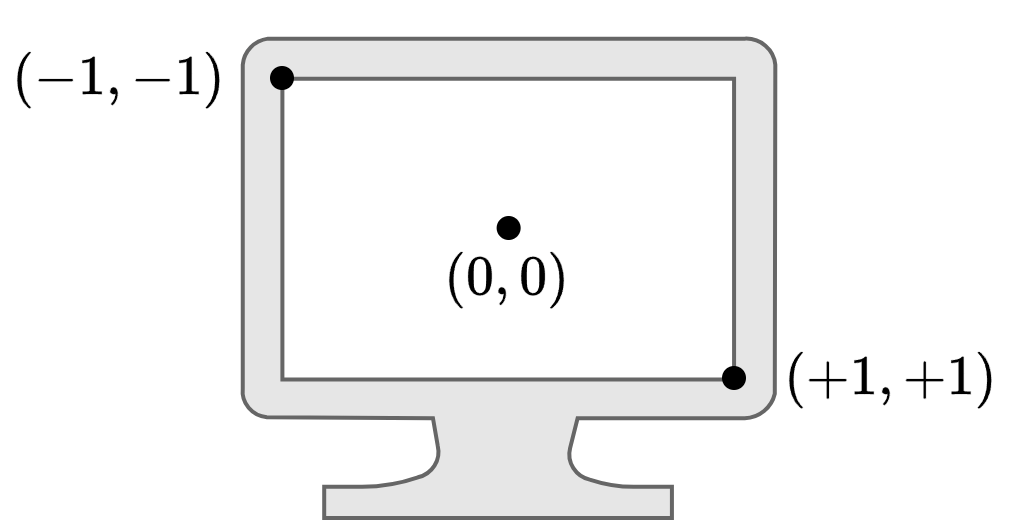
\includegraphics[width=0.5\linewidth]{images/nsc.png}
    \caption{Normalized screen coordinates}
\end{figure}
For example, both OpenGL and Vulkan employ normalized screen coordinates within the $\left[-1, 1\right]$ range.
However, OpenGL's $y$-axis increases upwards, while Vulkan adheres to the convention of pixel coordinates with the $y$-axis descending downwards.

Given a screen (or window, or memory area) resolution of $s_w \times s_h$ pixels. 
Pixel coordinates $\left(x_s,y_s\right)$ can be derived from normalized screen coordinates $\left(x_n,y_n\right)$ using a straightforward relation.
For Vulkan, the transformation is expressed as:
\[\begin{cases}
    x_s = (s_w-1) \cdot \dfrac{x_n+1}{2} \\ 
    y_s = (s_h-1) \cdot \dfrac{y_n+1}{2}
\end{cases}\]
As mentioned, screen buffers are typically accessed through their drivers and specific software libraries.
Programs generally utilize normalized screen coordinates, except in cases where they operate at a low level and must directly interact with the frame buffer.

\subsection{Graphics primitives}
Procedures responsible for drawing simple geometric shapes on a screen, utilizing a 2D coordinate system, are known as 2D graphics primitives.
Modern graphics adapters facilitate drawing operations by supporting three fundamental types of primitives: points, lines, and filled triangles.

These primitives work by manipulating and connecting points on the screen, identified by a pair of coordinates defined with a two-component vector. 
These coordinates are integer values measured in pixels.
The primitives employed for screen drawing (or within windows) automatically handle the calculations to determine the appropriate pixels on the screen based on normalized screen coordinates.

\paragraph*{Point}
Drawing a point entails setting the color of a pixel at a specified position on the screen. 
The graphic primitive responsible for this action is typically called \texttt{plot ()}. 
It requires parameters such as the coordinates of the pixel to be set $(x,y)$ and its color $(r,g,b)$.
\begin{figure}[H]
    \centering
    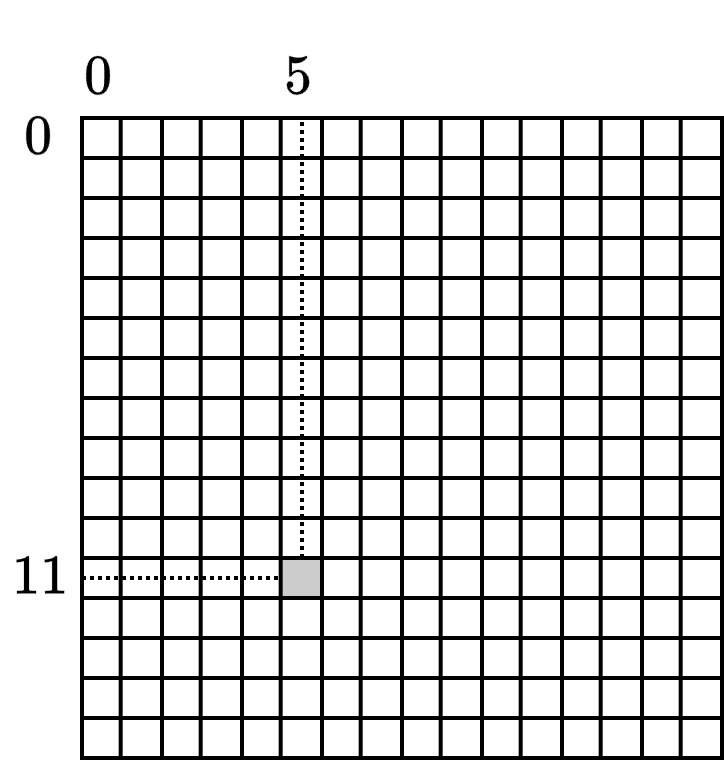
\includegraphics[width=0.35\linewidth]{images/plot.png}
    \caption{\texttt{plot (x:-0.312, y:0.562, r:0.8, g:0.8, b:0.8)}}
\end{figure}

\paragraph*{Line}
The line primitive connects two points on the screen with a straight segment. 
It necessitates the coordinates $(x_0,y_0)$ of the starting point and $(x_1,y_1)$ of the end point, along with the color definition.
\begin{figure}[H]
    \centering
    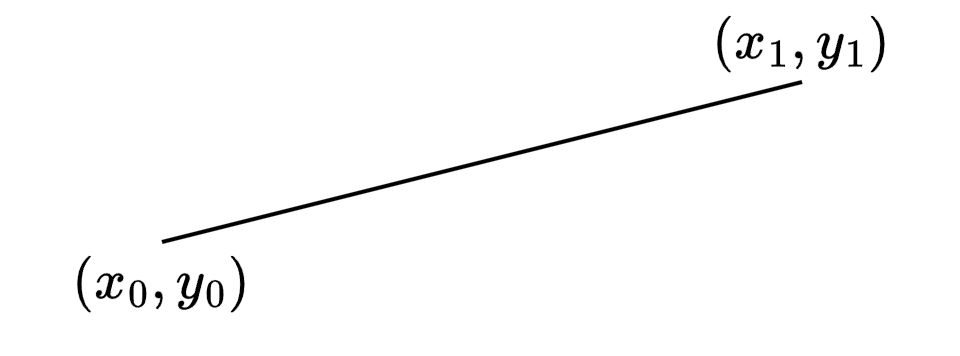
\includegraphics[width=0.4\linewidth]{images/line.png}
    \caption{Line primitive}
\end{figure}

\paragraph*{Filled triangle}
Filled triangles serve as the foundation of 3D computer graphics. 
They are defined by the coordinates of their three vertices $(x_0,y_0)$, $(x_1,y_1)$, and $(x_2,y_2)$, along with their corresponding color $(r,g,b)$.
\begin{figure}[H]
    \centering
    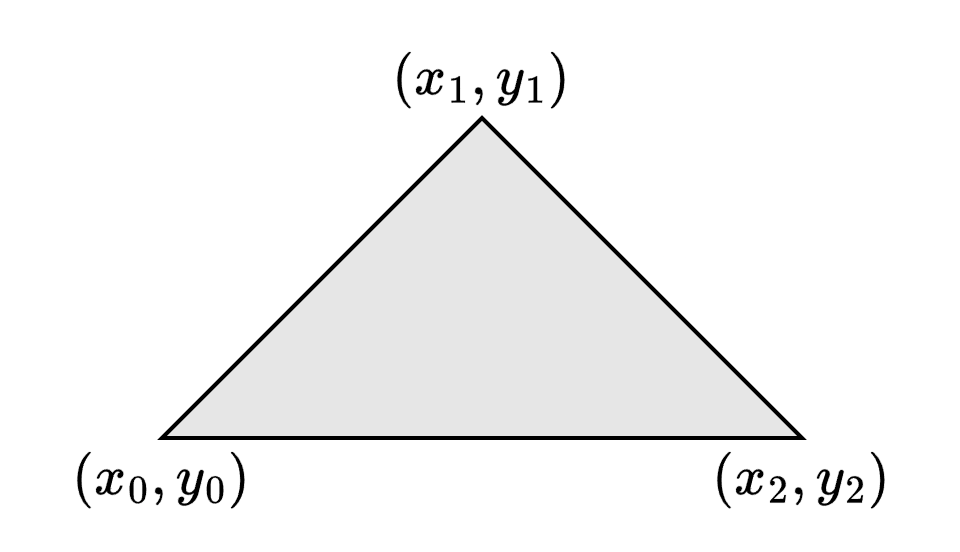
\includegraphics[width=0.4\linewidth]{images/triangle.png}
    \caption{Filled triangle primitive}
\end{figure}